\chapter{Detecting and shifting the bank lines} \label{Chp:BankDetect}

This chapter describes the algorithms used for detecting (see \autoref{Sec:BankDetect}) and shifting (see \autoref{Sec:BankShift}) the bank lines.
The former happens in the 'banklines' detection step, whereas the latter happens in the 'bankerosion' analysis step after the bank erosion rates have been computed.
It also lists issues that you may run into during the detection step (see \autoref{Sec:DetectIssues}).

\section{Detecting the bank lines} \label{Sec:BankDetect}

The location of bank lines is determined by identifying the boundary between water (wet) and land (dry) at a reference discharge computed using \dflowfm.
The detection of the bank lines builds on the search lines provided as input to this step.
The model domain is first clipped to the area close to the search lines (i.e.~within the user specified search distance from the search line) to focus the bank detection algorithm on the areas of interest only.
Identifying the exact location of the bank lines starts by determining for each grid cell in the area of interest whether it has one (or more) bed levels $z_b$ (defined at the mesh nodes) above the water level $z_w$ in the grid cell and one (or more) bed levels below the water level (see \autoref{Fig:detect_step}).

\Note \dfastbe currently only supports results of hydrodynamic simulations which use bed levels $z_b$ defined at grid nodes.
Simulations with bed levels defined in cell centres (tile depth) are thus not supported.

\begin{figure}[!h]
\center
\resizebox{5cm}{!}{
   \input{figures/detect_step.pdf_tex}
}
\caption{The bank line determined by the transition from wet (bed levels $z_b$ below water level $z_w$) to dry (bed levels $z_b$ above water level $z_w$) per triangle}
\label{Fig:detect_step}
\end{figure}

For each of those grid cells, the sub-grid boundary between dry and wet parts is determined as the line along which the interpolated bed level equals the water level in the grid cell.
The line marking the zero water depth is a straight line in a triangle.
Cells with $N_c \ge 4$ corners are split into $N_c - 2$ triangles to arrive at a collection of only straight line segments.
The collection of all these line segments forms the basis of the final bank line, which is obtained by connecting the individual segments into long connected strands.
Subsequently, those bank line strands are selected that are closest to the river axis (to avoid selecting banks of floodplain lakes or side channels that are located close to the bank of interest).
The selected strands are finally connected across side channels entrances and other gaps to a continuous bank line for the whole reach of interest.
The resulting lines are written to a shape file for checking and use in the 'bankerosion' analysis step.

The found locations of the bank lines will clearly depend on the chosen discharge level.
However, as long as the discharge is within the main channel, the locations will be fairly consistent.

Generally, bank erosion only occurs along the main channel.
It is therefore possible to only take into account those cells that are within a certain distance from the predefined search lines.
This is also necessary when more than one bank line is present (as is common in rivers), because otherwise it is not clear which coordinates belong to one bank or the other.

The search lines should be defined in a simple text file consisting of x- and y- coordinates (\command{Line1}, ..., \command{LineN}, in the configuration file).
For the Dutch rivers the lines can be obtained from the Baseline 'oeverlijnen' for model schematisations up to Baseline 4.
For model schematisations of Baseline 5 and higher the 'oeverlijnen' can be obtained by:
%
\begin{enumerate}
\item merging the baseline section 1 and 2 polygon in one polygon feature,
\item transferring this polygon to a polyline feature,
\item cutting this feature into two separate banklines, and
\item transforming these lines to points along the lines with an interval of 10 metres.
\end{enumerate}

By using the 'oeverlijnen', or section 1-2 boundary from Baseline the tool only depicts the main channel.
Possible side channels, shortcuts or lakes will not be detected by the tool, see \autoref{Fig3.2}.
If they are important, extra lines can be added that indicate the location of the bank lines of these individual features.
For this the input \command{NBank} should be increased by the number of extra features and the location of the bank line file \command{LineN} should point to the new file(s) with the xy-coordinates of extra search line(s).
It should be noted that for the analysis of these extra bank sections the tool will still use the closest point \emph{of the main channel} for which the fairway and river axis have been specified which is likely not correct.
Hence a better approach is to run a separate analysis for these reaches in which provide appropriate lines for the fairway and river axis of those side channels.

Groynes are not detected as such by the tool, because they are typically defined on sub-grid level in the simulations, see \autoref{Fig3.3}.
The detected bank line is in this case following the banks within groyne sections.
This is an advantage, since possible bank erosion only takes place in the groyne sections and not along the groynes themselves.

\begin{figure}[!h]
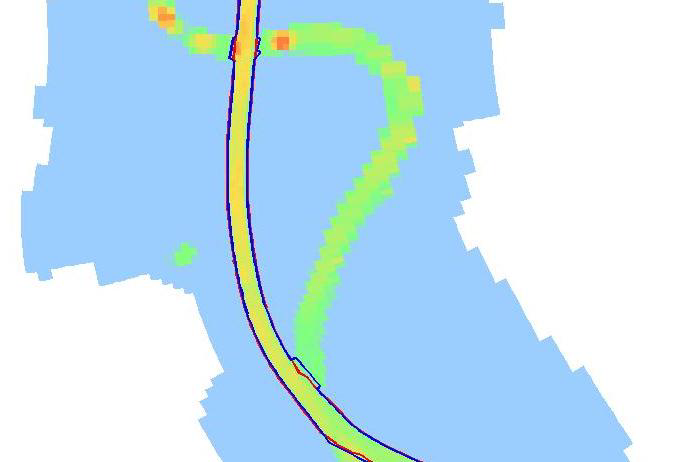
\includegraphics[width=\textwidth,height=7cm]{figures/Fig3-2.png}
\caption{Detection of bank lines at a shortcut in the Meuse river.
Red: Baseline 'section 1-2 boundary', Blue: detected bank line from WAQUA computation}
\label{Fig3.2}
\end{figure}

\begin{figure}[!hb]
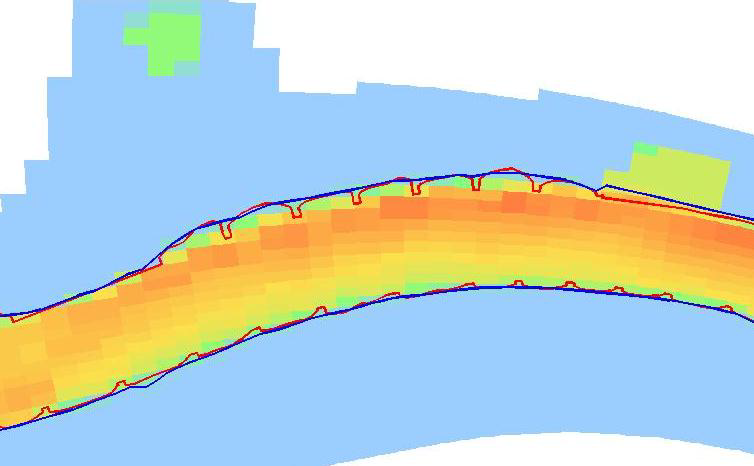
\includegraphics[width=\textwidth,height=7cm]{figures/Fig3-3.png}
\caption{Detection of a bank line close to groynes}
\label{Fig3.3}
\vspace{-0.75cm} 
\end{figure}
\clearpage

\section{Common issues with bank line detection} \label{Sec:DetectIssues}
It is advised to check the detected bank lines shown in the graphical output of the 'banklines' mode before continuing with the 'bankerosion' mode.
This section describes some common issues and their solutions.

\subsection{Detection of adjacent water body}
At some locations an adjacent water body is located within the given search distance from the predefined bank lines (parameter \command{Dlines}).
As a result the bank line of the adjacent water body is found, instead of the bank line of the main river channel.
As a result the initial bank line shows strange variations.
This is the case between kilometre 20 and 21 in \autoref{Fig_issue_bankline} location A.

\begin{figure}[!hb]
	\center
	\resizebox{15cm}{!}{
		\input{figures/detection_issue.pdf_tex}
	}
	\caption{Detection of the initial bank line close to adjacent water bodies}
	\label{Fig_issue_bankline}
\end{figure}

By decreasing the parameter \command{Dlines} you decrease the search distance from the predefined lines for determining the bank lines.
As a result, you decrease the chance that the bank line of an adjacent water  body is found.
However, you won't find a correct initial bank line if you make the parameter \command{Dlines} too small, this can be especially the case close to groins, at wide shallow areas or along banks with a relatively flat slope (see left bank between kilometre 22 and 23 in \autoref{Fig_issue_bankline} location B).

Another option is to edit the initial bank line manually by removing the points that fall in the adjacent water body, so only the points along the main channel remain.

\subsection{Irregularities in the detected bank line}
\autoref{Fig_issue_bankline} location C shows at the right outer bank after kilometre 22.5 a strange irregularity in the detected initial bank line.
This type of irregularities develop either by the detection of adjacent water body's, by the cut-off of connections with side channels (see \autoref{Fig_issue_bankline2}) or harbours or other irregularities along the bank.
It is advised to edit the initial bank line manually by removing some of the points so a smooth bank line along the main channel remains, because these irregularities influence the distance between the bank and the fairway and thus result in strange irregular patterns in wave heights and erosion along that bank.

\begin{figure}[!h]
	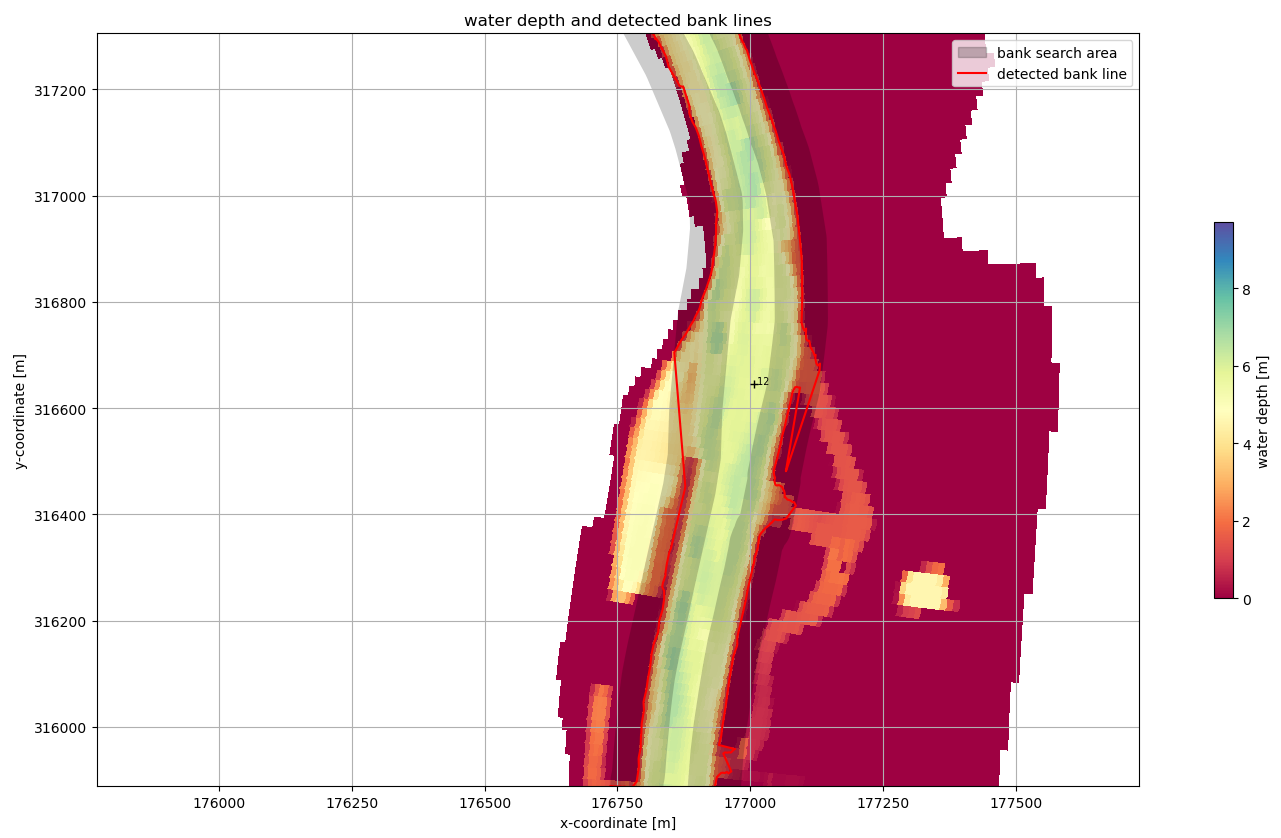
\includegraphics[width=\textwidth]{figures/detection_issue2.png}
	\caption{Detection of the initial bank line at the connection with a side channel}
	\label{Fig_issue_bankline2}
\end{figure}

\section{Shifting the bank lines} \label{Sec:BankShift}

The new location of the bank line is determined by shifting each bank line segment individually by its local erosion distance.
In the case of a concave bend the eroding segments move apart; a new bank segment is inserted connecting the two end points of the previously connected segments (see \autoref{Fig:erode_shift}, subplot a).
In case of a convex bend the eroding segments overlap; in this case the new bank line follows the outline of furthest erosion (see subplot b).

\begin{figure}[!h]
\center
\resizebox{12cm}{!}{
   \input{figures/erode_shift_step.pdf_tex}
}
\caption{Shifting a bank line first moves each line segment, and subsequently adds or removes segments as necessary}
\label{Fig:erode_shift}
\end{figure}
